% ******************************* Master Thesis Template **************************
% Please have a look at the README.txt file for info on how to use the template

\documentclass[a4paper,custommargin,times,numbered,langen,printindex]{Classes/UCMScRProj}

% ******************************************************************************
% ******************************* Class Options ********************************
% *********************** See README for more details **************************
% ******************************************************************************
% *********************** RECOMMENDATIONS **************************************

% `a4paper'
%
% `11pt'�(default): Font Size 12pt is NOT recommended.

% ********************** SOME OPTIONS ******************************************
%
% `oneside' or `twoside'(default): Printing double side (twoside) or single
% side.
%
% `print': Use `print' for print version with appropriate margins and page
% layout. Leaving the options field blank will activate Online version.
%
% `langen`: This redefines the style to English language if the MSc Thesis is written in English.
%  The default language is Portuguese. In this case of using Portuguese there is no need to declare it.
%
% `index': For index at the end of the thesis
%
% `draft': For draft mode without loading any images (same as draft in book)
%
% `draftmode': Special draft mode with line numbers, images, and water mark with
% timestamp and custom text. Position of the text can also be modified.
%
% `abstract': To generate only the title page and abstract page with
% dissertation title and name.
%
% `chapter`: This option enables only the specified chapter and it's references
%  Useful for review and corrections.
%
% ************************* Custom Page Margins ********************************
%
% `custommargin`: Use `custommargin' in options to activate custom page margins,
% which can be defined in the preamble.tex. Custom margin will override
% print/online margin setup.
%
% *********************** Choosing the Fonts in Class Options ******************
%
% `times' : Times font with math support.
%
% `fourier': Utopia Font with Fourier Math font (Font has to be installed)
%            It's a free font.
%
% `customfont': Use `customfont' option in the document class and load the
% package in the preamble.tex
%
% default or leave empty: `Latin Modern' font will be loaded.
%
% ********************** Choosing the Bibliography style ***********************
%
% `authoryear': For author-year citation eg., Krishna (2013)
%
% `numbered': (Default Option) For numbered and sorted citation e.g., [1,5,2]
%
% `custombib': Define your own bibliography style in the `preamble.tex' file.
%              `\RequirePackage[square, sort, numbers, authoryear]{natbib}'.
%              This can be also used to load biblatex instead of natbib
%              (See Preamble)
%
% **************************** Choosing the Page Style *************************
%
% `default (leave empty)': For Page Numbers in Header (Left Even, Right Odd) and
% Chapter Name in Header (Right Even) and Section Name (Left Odd). Blank Footer.
%
% `PageStyleI': Chapter Name next & Page Number on Even Side (Left Even).
% Section Name & Page Number in Header on Odd Side (Right Odd). Footer is empty.
%
% `PageStyleII': Chapter Name on Even Side (Left Even) in Header. Section Number
% and Section Name in Header on Odd Side (Right Odd). Page numbering in footer


% ********************************** Preamble **********************************
% Preamble: Contains packages and user-defined commands and settings
% ******************************************************************************
% ****************************** Custom Margin *********************************

% Add `custommargin' in the document class options to use this section
% Set {innerside margin / outerside margin / topmargin / bottom margin}  and
% other page dimensions
\ifsetCustomMargin
  \RequirePackage[left=28mm,right=28mm,top=35mm,bottom=30mm]{geometry}
  \setFancyHdr % To apply fancy header after geometry package is loaded
\fi

% *****************************************************************************
% ******************* Fonts (like different typewriter fonts etc.)*************

% Add `customfont' in the document class option to use this section

\ifsetCustomFont
  % Set your custom font here and use `customfont' in options. Leave empty to
  % load computer modern font (default LaTeX font).
  \RequirePackage{helvet}
\fi

% *****************************************************************************
% ******************* COVER / CAPA ********************************************
\usepackage{pdfpages}

% *****************************************************************************
% **************************** Custom Packages ********************************

\usepackage[all]{xypic}
%\usepackage{algpseudocode}


% ********************Captions and Hyperreferencing / URL **********************

% Captions: This makes captions of figures use a boldfaced small font.
%\RequirePackage[small,bf]{caption}

\RequirePackage[labelsep=space,tableposition=top]{caption}
\renewcommand{\figurename}{Fig.} %to support older versions of captions.sty


% *************************** Graphics and figures *****************************

%\usepackage{rotating}
%\usepackage{wrapfig}

% Uncomment the following two lines to force Latex to place the figure.
% Use [H] when including graphics. Note 'H' instead of 'h'
%\usepackage{float}
%\restylefloat{figure}

% Subcaption package is also available in the sty folder you can use that by
% uncommenting the following line
% This is for people stuck with older versions of texlive
%\usepackage{sty/caption/subcaption}
\usepackage{subcaption}

% ********************************** Tables ************************************
\usepackage{booktabs} % For professional looking tables
\usepackage{multirow}

%\usepackage{multicol}
%\usepackage{longtable}
%\usepackage{tabularx}


% ***************************** Math ******************************

\usepackage{amsfonts}
\usepackage{amsmath}
\usepackage{amssymb}
\usepackage{stmaryrd} % \mapsfrom

%%%%%%%%%%
%%% Listagens
%%%%%%%%%%
\usepackage{listingsutf8}

\renewcommand{\lstlistingname}{Algoritmo}% Listing -> Algorithm
\renewcommand{\lstlistlistingname}{Lista de \lstlistingname s}% List of Listings -> List of Algorithms


 % definição da linguagem de programação
\lstset{language=C++,
  extendedchars=true,
  inputencoding=utf8,
  morekeywords={typedef,cin,cout,NULL,FILE},
  basicstyle=\small,
  frame=single
}

%  % definição da linguagem de programação
\lstdefinelanguage{algoritmo}{
  keywords={enquanto,para,se,entao,senao,fimse,fimpara,fimenquanto,faz,funcao,fimfuncao,return},
   extendedchars=true,
   inputencoding=utf8,
   morekeywords={faz,funcao,return},
   basicstyle=\small,
   frame=single
}

% para lidar com o UTF8
\lstset{literate=
  {á}{{\'a}}1 {é}{{\'e}}1 {í}{{\'i}}1 {ó}{{\'o}}1 {ú}{{\'u}}1
  {Á}{{\'A}}1 {É}{{\'E}}1 {Í}{{\'I}}1 {Ó}{{\'O}}1 {Ú}{{\'U}}1
  {à}{{\`a}}1 {è}{{\`e}}1 {ì}{{\`i}}1 {ò}{{\`o}}1 {ù}{{\`u}}1
  {À}{{\`A}}1 {È}{{\'E}}1 {Ì}{{\`I}}1 {Ò}{{\`O}}1 {Ù}{{\`U}}1
  {ä}{{\"a}}1 {ë}{{\"e}}1 {ï}{{\"i}}1 {ö}{{\"o}}1 {ü}{{\"u}}1
  {Ä}{{\"A}}1 {Ë}{{\"E}}1 {Ï}{{\"I}}1 {Ö}{{\"O}}1 {Ü}{{\"U}}1
  {â}{{\^a}}1 {ê}{{\^e}}1 {î}{{\^i}}1 {ô}{{\^o}}1 {û}{{\^u}}1
  {Â}{{\^A}}1 {Ê}{{\^E}}1 {Î}{{\^I}}1 {Ô}{{\^O}}1 {Û}{{\^U}}1
  {Ã}{{\~A}}1 {ã}{{\~a}}1 {Õ}{{\~O}}1 {õ}{{\~o}}1 {ñ}{{\~n}}1
  {œ}{{\oe}}1 {Œ}{{\OE}}1 {æ}{{\ae}}1 {Æ}{{\AE}}1 {ß}{{\ss}}1
  {ű}{{\H{u}}}1 {Ű}{{\H{U}}}1 {ő}{{\H{o}}}1 {Ő}{{\H{O}}}1
  {ç}{{\c c}}1 {Ç}{{\c C}}1 {«}{{\guillemotleft}}1 {»}{{\guillemotright}}1
  {€}{{\EUR}}1 {£}{{\pounds}}1
}


% ******************************* Line Spacing *********************************

% Choose linespacing as appropriate. Default is one-half line spacing

% \doublespacing
% \onehalfspacing
% \singlespacing


% ************************ Formatting / Footnote *******************************

% Don't break enumeration (etc.) across pages in an ugly manner (default 10000)
%\clubpenalty=500
%\widowpenalty=500

%\usepackage[perpage]{footmisc} %Range of footnote options


% *****************************************************************************
% *************************** Bibliography  and References ********************

%\usepackage{cleveref} %Referencing without need to explicitly state fig /table

% Add `custombib' in the document class option to use this section
\ifuseCustomBib
   \RequirePackage[square, sort, numbers, authoryear]{natbib} % CustomBib

% If you would like to use biblatex for your reference management, as opposed to the default `natbibpackage` pass the option `custombib` in the document class. Comment out the previous line to make sure you don't load the natbib package. Uncomment the following lines and specify the location of references.bib file

%\RequirePackage[backend=biber, style=numeric-comp, citestyle=numeric, sorting=nty, natbib=true]{biblatex}
%\bibliography{References/references} %Location of references.bib only for biblatex

\fi

% changes the default name `Bibliography` -> `References'
\ifisLangPt
  \renewcommand{\bibname}{Bibliografia}
\else
  \renewcommand{\bibname}{References}
\fi


% *****************************************************************************
% *************** Changing the Visual Style of Chapter Headings ***************

% Uncomment the section below. Requires titlesec package.

%\RequirePackage{titlesec}
%\newcommand{\PreContentTitleFormat}{\titleformat{\chapter}[display]{\scshape\Large}
%{\Large\filleft{\chaptertitlename} \Huge\thechapter}
%{1ex}{}
%[\vspace{1ex}\titlerule]}
%\newcommand{\ContentTitleFormat}{\titleformat{\chapter}[display]{\scshape\huge}
%{\Large\filleft{\chaptertitlename} \Huge\thechapter}{1ex}
%{\titlerule\vspace{1ex}\filright}
%[\vspace{1ex}\titlerule]}
%\newcommand{\PostContentTitleFormat}{\PreContentTitleFormat}
%\PreContentTitleFormat


% ******************************************************************************
% ************************* User Defined Commands ******************************
% ******************************************************************************

% *********** To change the name of Table of Contents / LOF and LOT ************

%\renewcommand{\contentsname}{My Table of Contents}
%\renewcommand{\listfigurename}{My List of Figures}
%\renewcommand{\listtablename}{My List of Tables}


% ********************** TOC depth and numbering depth *************************

\setcounter{secnumdepth}{2}
\setcounter{tocdepth}{2}


% ******************************* Nomenclature *********************************

% To change the name of the Nomenclature section, uncomment the following line

%\renewcommand{\nomname}{List of Symbols}


% ********************************* Appendix ***********************************

% The default value of both \appendixtocname and \appendixpagename is `Appendices'. These names can all be changed via:

%\renewcommand{\appendixtocname}{List of appendices}
%\renewcommand{\appendixname}{Appndx}
\ifisLangPt
  \renewcommand{\appendixname}{Anexo}
%  \renewcommand{\appendixtocname}{Lista de Ap\textasciicircum endices}
\fi

% ******************************** Draft Mode **********************************

% Uncomment to disable figures in `draftmode'
%\setkeys{Gin}{draft=true}  % set draft to false to enable figures in `draft'

% These options are active only during the draft mode
% Default text is "Draft"
%\SetDraftText{DRAFT}

% Default Watermark location is top. Location (top/bottom)
%\SetDraftWMPosition{bottom}

% Draft Version - default is v1.0
%\SetDraftVersion{v1.1}

% Draft Text grayscale value (should be between 0-black and 1-white)
% Default value is 0.75
%\SetDraftGrayScale{0.8}


%% Todo notes functionality
%% Uncomment the following lines to have todonotes.

%\ifsetDraft
%	\usepackage[colorinlistoftodos]{todonotes}
%	\newcommand{\mynote}[1]{\todo[author=kks32,size=\small,inline,color=green!40]{#1}}
%\else
%	\newcommand{\mynote}[1]{}
%	\newcommand{\listoftodos}{}
%\fi

% Example todo: \mynote{Hey! I have a note}




% ************************ Thesis Information & Meta-data **********************
% Thesis title and author information, reference file for biblatex

% ************************ Thesis Information **********************
%% The title of the thesis
\title{Criptografia RSA}

%% The full name of the author
\author{José Diogo Songo}

%% Logo
\crest{
\includegraphics[width=0.4\textwidth]{UC_fundoclaro.png}}

%% Uncomment the appropriate lines
\spareaLangEn{Applied Analysis and Computation}
%\spareaLangEn{Statistics, Optimization and Mathematics in Finance}
%\spareaLangEn{Pure Mathematics}
\spareaLangPt{An\'{a}lise Aplicada e Computa\c{c}\~{a}o}
%\spareaLangPt{Estat\'{\i}stica, Otimiza\c{c}\~{a}o e Matem\'{a}tica Financeira}
%\spareaLangPt{Matem\'{a}tica Pura}

%% Full title of the Program
\ifisLangEn
  \degree{Research Seminar \\[2mm] Seminário de Investigação}
\else
  \degree{Seminário de Investigação \\[2mm] Research Seminar}
\fi


%% Submission date
% Default is set as {\monthname[\the\month]\space\the\year}
%%
%% Uncomment the appropriate line and update with the actual defense date in the given format
%%
%\degreedate{September 2016}
%\degreedate{Janeiro 2019 / January 2019}
\ifisLangEn
  \degreedate{January 2024 / Janeiro 2024}
\else
  \degreedate{Janeiro 2024 / January 2024}
\fi


% ***************************** Abstract Separate ******************************
% To printout only the titlepage and the abstract with the MSc title and the
% author name for submission to the Registry, use the `abstract' option in
% the document class.

\ifdefineAbstract
 \pagestyle{empty}
 \includeonly{Abstract/abstract}
\fi

% ***************************** Chapter Mode ***********************************
% The chapter mode allows user to only print particular chapters with references
% Title, Contents, Frontmatter are disabled by default
% Useful option to review a particular chapter or to send it to supervisor.
% To use choose `chapter' option in the document class

\ifdefineChapter
 \includeonly{Chapter3/chapter3}
\fi

% ******************************** Front Matter ********************************
\begin{document}

% COVER UC
% The cover should be prepared in the University template (file 'Capa_Dissertacao_TPL-A4.docx') and saved as a pdf file to include here
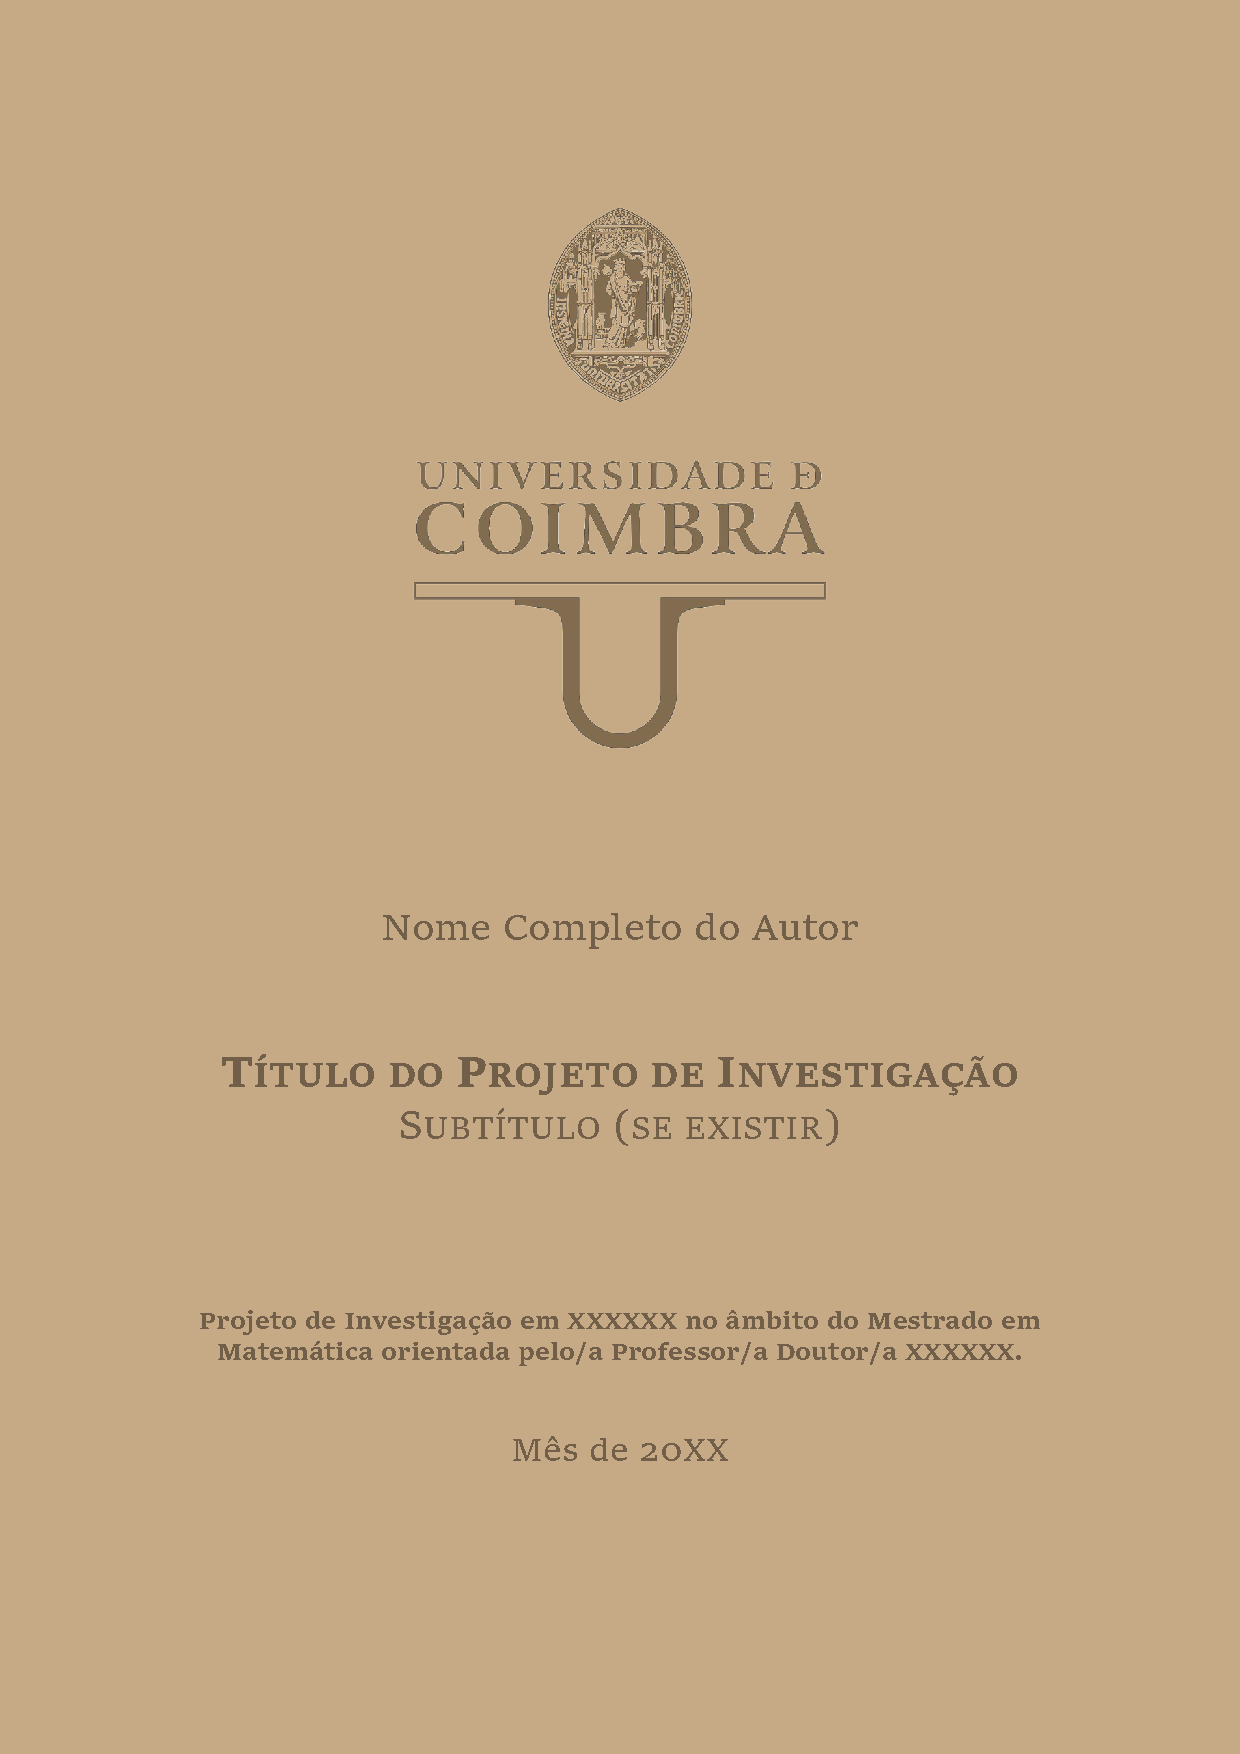
\includepdf{Cover/Capa_Dissertacao_TPL-A4.pdf}


\frontmatter

\begin{titlepage}
  \vspace*{30mm}
  \maketitle
\end{titlepage}


% ************************** Thesis Acknowledgements *****************************

\begin{acknowledgements}


Agradeço ao professor Pedro Quaresma, que aceitou orientar o meu projeto, revelando uma especial atenção às minhas ideias. Os seus conselhos e sugestões bem como a valorização do trabalho desenvolvido foram determinantes para alcançar este resultado.


\end{acknowledgements}

% ************************** Thesis Abstract *****************************
% Use `abstract' as an option in the document class to print only the titlepage and the abstract.
\begin{abstract}
\ifisLangEn

If the Dissertation is in Portuguese, do not write here anything.
This is where you write your abstract in English.

% ************************************************************************
%
% As linhas seguintes definem o `resumo' em portugu\^{e}s apenas no caso
% da l\'{\i}ngua utilizada ser o ingl\^{e}s. Caso contr\'{a}rio, ser\~{a}o ignoradas.
%
% ************************************************************************

  \cleardoublepage
  \setsinglecolumn
  \chapter*{\centering \Large Resumo}
  \thispagestyle{empty}

\else
  %Aqui escreve o Resumo em Portugu\^{e}s no caso da disserta\c{c}\~{a}o usar o Ingl\^{e}s.

    A criptografia RSA revolucionou a segurança digital com o seu procedimento de chaves pública e privada, em contraponto com as cifras de chaves simétricas cuja gestão das chaves é muito difícil de gerir em ambientes com muitos intervenientes. A criptoanálise, por sua vez, desempenha um papel fundamental na avaliação e no aprimoramento da segurança dos sistemas criptográficos, buscando constantemente formas de tornar as comunicações digitais mais seguras e protegidas contra ameaças cibernéticas.

    Neste texto apresentam-se as implementações dos diferentes métodos descritos no trabalho de seminário, nomeadamente, os algoritmos para os métodos de deslocamento simples, linear e RSA.
    
    No final, foi feito um estudo comparativo dos métodos acima mencionados.
\fi
\end{abstract}


% *********************** Adding TOC and List of Figures ***********************

\tableofcontents

\listoffigures

\listoftables

% *********************** Index of Nomenclature (Optional) ***********************
%
%% printnomencl should be commented out, if you are using a list of Nomenclature
%
% ********************************************************************************

%% In case you don�t like the name of the nomenclature, just redefine the \nomname macro, e. g.
%\renewcommand{\nomname}{List of symbols}

%\printnomencl

%% It uses the package nomencl
%%\printnomencl[space] space can be set as 2em between symbol and description
%%\printnomencl[3em]

%%%% IMPORTANT: The nomencl package only creates a fyle thesis.nlo.
%%%%            You need to create the file thesis.nls that contains your nomenclature list properly ordered.
%%
%% In order to do that and to include the list in the pdf the compile sequence must be:
%% run pdfLaTeX
%% run makeindex thesis.nlo -s nomencl.ist -o thesis.nls
%% then rerun pdfLaTeX


% ******************************** Main Matter *********************************
\mainmatter

%*******************************************************************************
%*********************************** First Chapter *****************************
%*******************************************************************************

\chapter{Introduction}   %Title of the First Chapter

\ifpdf
    \graphicspath{{Chapter1/Figs/Raster/}{Chapter1/Figs/PDF/}{Chapter1/Figs/}}
\else
    \graphicspath{{Chapter1/Figs/Vector/}{Chapter1/Figs/}}
\fi


%********************************** %First Section  **************************************
\section{First section of the first chapter}

And now I begin my first chapter here \dots

And now to cite some people~\citet{Rea85,Ancey1996}

How to index a name:

A {\em \LaTeX{} class file}\index{\LaTeX{} class file@LaTeX class file} is a file, which holds style information for a particular \LaTeX{}.

How to start a list of Nomenclature and Notation (OPTIONAL): ...


\nomenclature[z-cif]{$CIF$}{Cauchy's Integral Formula}                                % first letter Z is for Acronyms
\nomenclature[a-F]{$F$}{complex function}                                                   % first letter A is for Roman symbols
\nomenclature[g-p]{$\pi$}{ $\simeq 3.14\ldots$}                                             % first letter G is for Greek Symbols
\nomenclature[g-i]{$\iota$}{unit imaginary number $\sqrt{-1}$}                      % first letter G is for Greek Symbols
\nomenclature[g-g]{$\gamma$}{a simply closed curve on a complex plane}  % first letter G is for Greek Symbols
\nomenclature[x-i]{$\oint_\gamma$}{integration around a curve $\gamma$} % first letter X is for Other Symbols
\nomenclature[r-j]{$j$}{superscript index}                                                       % first letter R is for superscripts
\nomenclature[s-0]{$0$}{subscript index}                                                        % first letter S is for subscripts


\subsection{First subsection in the first section}
\dots and some more

\subsection{Second subsection in the first section}
\dots and some more \dots

\subsubsection{First subsub section in the second subsection}
\dots and some more in the first subsub section otherwise it all looks the same
doesn't it? well we can add some text to it \dots

\subsection{Third subsection in the first section}
\dots and some more \dots

\subsubsection{First subsub section in the third subsection}
\dots and some more in the first subsub section otherwise it all looks the same
doesn't it? well we can add some text to it and some more and some more and
some more and some more and some more and some more and some more \dots

\subsubsection{Second subsub section in the third subsection}
\dots and some more in the first subsub section otherwise it all looks the same
doesn't it? well we can add some text to it \dots

%********************************** %Second Section  *************************************
\section{Second section of the first chapter}
and here I write more \dots

\section{The layout of formal tables}
This section has been modified from ``Publication quality tables in \LaTeX*''
 by Simon Fear.

The layout of a table has been established over centuries of experience and
should only be altered in extraordinary circumstances.

When formatting a table, remember two simple guidelines at all times (see Table \ref{table1}):

\begin{enumerate}
  \item Never, ever use vertical rules (lines).
  \item Never use double rules.
\end{enumerate}

These guidelines may seem extreme but I have
never found a good argument in favour of breaking them. For
example, if you feel that the information in the left half of
a table is so different from that on the right that it needs
to be separated by a vertical line, then you should use two
tables instead. Not everyone follows the second guideline:

There are three further guidelines worth mentioning here as they
are generally not known outside the circle of professional
typesetters and subeditors:

\begin{enumerate}\setcounter{enumi}{2}
  \item Put the units in the column heading (not in the body of
          the table).
  \item Always precede a decimal point by a digit; thus 0.1
      {\em not} just .1.
  \item Do not use `ditto' signs or any other such convention to
      repeat a previous value. In many circumstances a blank
      will serve just as well. If it won't, then repeat the value.
\end{enumerate}

A frequently seen mistake is to use `\textbackslash begin\{center\}' \dots `\textbackslash end\{center\}' inside a figure or table environment. This center environment can cause additional vertical space. If you want to avoid that just use `\textbackslash centering'

These guidelines may seem extreme but I have
never found a good argument in favour of breaking them. For
example, if you feel that the information in the left half of
a table is so different from that on the right that it needs
to be separated by a vertical line, then you should use two
tables instead. Not everyone follows the second guideline:

There are three further guidelines worth mentioning here as they
are generally not known outside the circle of professional
typesetters and subeditors:


\begin{table}
\caption{A badly formatted table}
\centering
\label{table:bad_table}
\begin{tabular}{|l|c|c|c|c|}
\hline
& \multicolumn{2}{c}{Species I} & \multicolumn{2}{c|}{Species II} \\
\hline
Dental measurement  & mean & SD  & mean & SD  \\ \hline
\hline
I1MD & 6.23 & 0.91 & 5.2  & 0.7  \\
\hline
I1LL & 7.48 & 0.56 & 8.7  & 0.71 \\
\hline
I2MD & 3.99 & 0.63 & 4.22 & 0.54 \\
\hline
I2LL & 6.81 & 0.02 & 6.66 & 0.01 \\
\hline
CMD & 13.47 & 0.09 & 10.55 & 0.05 \\
\hline
CBL & 11.88 & 0.05 & 13.11 & 0.04\\
\hline
\end{tabular}
\end{table}

\begin{table}
\caption{A nice looking table}
\centering
\label{table:nice_table}
\begin{tabular}{l c c c c}
\hline
\multirow{2}{*}{Dental measurement} & \multicolumn{2}{c}{Species I} & \multicolumn{2}{c}{Species II} \\
\cline{2-5}
  & mean & SD  & mean & SD  \\
\hline
I1MD & 6.23 & 0.91 & 5.2  & 0.7  \\

I1LL & 7.48 & 0.56 & 8.7  & 0.71 \\

I2MD & 3.99 & 0.63 & 4.22 & 0.54 \\

I2LL & 6.81 & 0.02 & 6.66 & 0.01 \\

CMD & 13.47 & 0.09 & 10.55 & 0.05 \\

CBL & 11.88 & 0.05 & 13.11 & 0.04\\
\hline
\end{tabular}
\end{table}


\begin{table}
\caption{Even better looking table using booktabs}
\centering
\label{table:good_table}
\begin{tabular}{l c c c c}
\toprule
\multirow{2}{*}{Dental measurement} & \multicolumn{2}{c}{Species I} & \multicolumn{2}{c}{Species II} \\
\cmidrule{2-5}
  & mean & SD  & mean & SD  \\
\midrule
I1MD & 6.23 & 0.91 & 5.2  & 0.7  \\

I1LL & 7.48 & 0.56 & 8.7  & 0.71 \\

I2MD & 3.99 & 0.63 & 4.22 & 0.54 \\

I2LL & 6.81 & 0.02 & 6.66 & 0.01 \\

CMD & 13.47 & 0.09 & 10.55 & 0.05 \\

CBL & 11.88 & 0.05 & 13.11 & 0.04\\
\bottomrule
\end{tabular}
\end{table}

\begin{table}
\caption{Characterizations of normal and extremally disconnected spaces}
\label{table1}
\begin{center}
\begin{tabular}{p{91pt}p{150pt}p{155pt}}
\toprule[1.2pt]   {\bf Space $\boldsymbol{X}$} &   {\sc Normal} &
{\sc Extremally Disconnected}  \\
\bottomrule[1.2pt]
\addlinespace[5pt]
\raggedright {\sf Urysohn's separation type lemma} & \raggedright Every two disjoint {\sc closed}\break subsets of $X$ are completely separated (Urysohn 1925). & \raggedright Every two disjoint {\sc open} subsets of $X$ are completely separated (Gillman \& Jerison 1960).\tabularnewline
\addlinespace[5pt]\midrule\addlinespace[5pt]
\raggedright {\sf Tietze's extension type theorem} & \raggedright Each {\sc closed} subset of $X$ is $C^*$-embedded (Tietze 1915). & \raggedright Each {\sc open} subset of $X$ is $C^*$-embedded (Gillman \& Jerison 1960). \tabularnewline
\addlinespace[5pt]\midrule\addlinespace[5pt]
\raggedright {\sf Kat\v{e}tov-Tong insertion type theorem} & For every {\sc upper} sem\-i\-con\-tin\-u\-ous real function $f$ and {\sc lower} sem\-i\-con\-tin\-u\-ous real function $g$ satisfying $f\le g$, there exists a continuous real function $h$ such that $f\le h\le g$ (Kat\v{e}tov 1951, Tong 1952). & For every {\sc lower} sem\-i\-con\-tin\-u\-ous real function $f$ and {\sc upper} sem\-i\-con\-tin\-u\-ous real function $g$ satisfying $f\le g$, there exists a continuous real function $h$ such that $f\le h\le g$ (Stone 1949, Lane 1975).\\
\addlinespace[5pt]\midrule\addlinespace[5pt]
\raggedright {\sf Hausdorff mapping invariance type theorem} & \raggedright The image of $X$ under any  {\sc closed} continuous map is {\sc normal} (Hausdorff 1935). & \raggedright
The image of $X$ under any {\sc open} continuous map is {\sc extremally disconnected}. \tabularnewline
\addlinespace[5pt]\bottomrule[1.2pt]
\end{tabular}
\end{center}
\end{table}

\section{Next section}

\section{Next section}



%*******************************************************************************
%****************************** Second Chapter *********************************
%*******************************************************************************

\chapter{My second chapter}

\graphicspath{{Chapter2/Figs/Box1/}{Chapter2/Figs/Box2/}}



\section[Short title]{Reasonably long section title}

I'm going to randomly include a picture in Figure~\ref{fig:Figure1}.

\bigskip
\begin{figure}[htbp!]
\centering
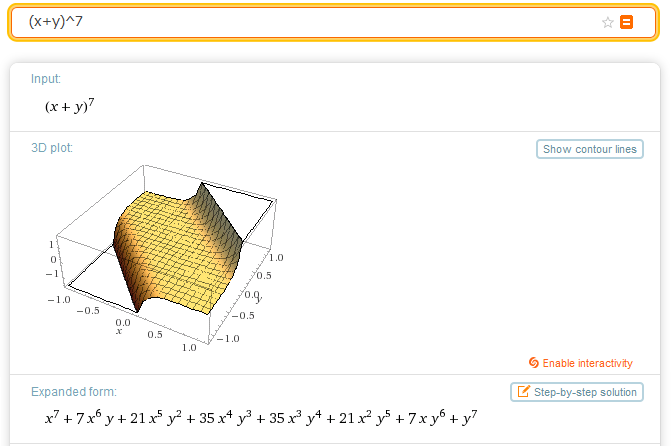
\includegraphics[width=1\textwidth]{alpha.png}
\caption[Figure 1]{This is just a long figure caption}
\label{fig:Figure1}
\end{figure}


\section*{Enumeration}
\begin{enumerate}
\item The first topic is dull
\item The second topic is duller
\begin{enumerate}
\item The first subtopic is silly
\item The second subtopic is stupid
\end{enumerate}
\item The third topic is the dullest
\end{enumerate}

\section*{itemize}
\begin{itemize}
\item The first topic is dull
\item The second topic is duller
\begin{itemize}
\item The first subtopic is silly
\item The second subtopic is stupid
\end{itemize}
\item The third topic is the dullest
\end{itemize}

\section*{description}
\begin{description}
\item[The first topic] is dull
\item[The second topic] is duller
\begin{description}
\item[The first subtopic] is silly
\item[The second subtopic] is stupid
\end{description}
\item[The third topic] is the dullest
\end{description}

\section{Second section}
Galois was born on 25 October 1811 to Nicolas-Gabriel Galois and Ad\'{e}la\"{\i}de-Marie (born Demante). His father was a Republican and was head of Bourg-la-Reine's liberal party. He became mayor of the village after Louis XVIII returned to the throne in 1814. His mother, the daughter of a jurist, was a fluent reader of Latin and classical literature and was responsible for her son's education for his first twelve years. At the age of 10, Galois was offered a place at the college of Reims, but his mother preferred to keep him at home.

In October 1823, he entered the Lyc\'{e}e Louis-le-Grand, and despite some turmoil in the school at the beginning of the term (when about a hundred students were expelled), Galois managed to perform well for the first two years, obtaining the first prize in Latin. He soon became bored with his studies and, at the age of 14, he began to take a serious interest in mathematics.

He found a copy of Adrien Marie Legendre's {\it \'{E}l\'{e}ments de G\'{e}om\'{e}trie}, which it is said that he read ``like a novel'' and mastered at the first reading. At 15, he was reading the original papers of Joseph Louis Lagrange, such as the landmark {\it R\'{e}flexions sur la r\'{e}solution alg\'{e}brique des \'{e}quations} which likely motivated his later work on equation theory, and {\it Le\c{c}ons sur le calcul des fonctions}, work intended for professional mathematicians, yet his classwork remained uninspired, and his teachers accused him of affecting ambition and originality in a negative way.\footnote{My footnote goes blah blah blah! \dots}.

While many mathematicians before Galois gave consideration to what are now known as groups, it was Galois who was the first to use the word group (in French {\it groupe}) in a sense close to the technical sense that is understood today, making him among the founders of the branch of algebra known as group theory. He developed the concept that is today known as a normal subgroup. He called the decomposition of a group into its left and right cosets a proper decomposition if the left and right cosets coincide, which is what today is known as a normal subgroup. He also introduced the concept of a finite field (also known as a Galois field in his honor), in essentially the same form as it is understood today.

In his last letter to Chevalier and attached manuscripts, the second of three, he made basic studies of linear groups over finite fields:

\begin{itemize}
    \item He constructed the general linear group over a prime field, $GL(\nu, p)$ and computed its order, in studying the Galois group of the general equation of degree $p^\nu$.
    \item He constructed the projective special linear group $PSL(2,p)$. Galois constructed them as fractional linear transforms, and observed that they were simple except if p was 2 or 3. These were the second family of finite simple groups, after the alternating groups.
    \item He noted the exceptional fact that $PSL(2,p)$ is simple and acts on $p$ points if and only if $p$ is 5, 7, or 11.
\end{itemize}


\begin{landscape}

\section*{Subplots}
I can cite AAA (see Fig.~\ref{fig:Collatz}) and BBB (Fig.~\ref{fig:Figure2}) or I can cite the whole figure as Fig.~\ref{fig:animations}


\begin{figure}
  \centering
  \begin{subfigure}[b]{0.55\textwidth}
    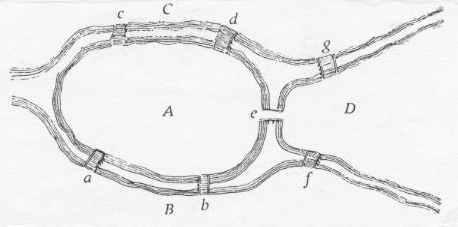
\includegraphics[width=\textwidth]{setepontes}
    \caption{7 Bridges}
    \label{fig:7 Bridges}
  \end{subfigure}
  \begin{subfigure}[b]{0.42\textwidth}
    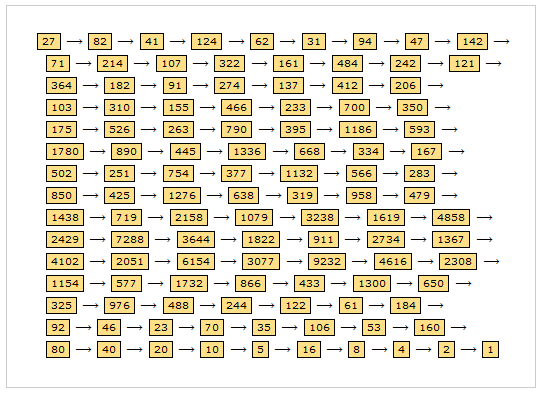
\includegraphics[width=\textwidth]{collatz}
    \caption{Collatz}
    \label{fig:Collatz}
  \end{subfigure}
  \begin{subfigure}[b]{0.42\textwidth}
    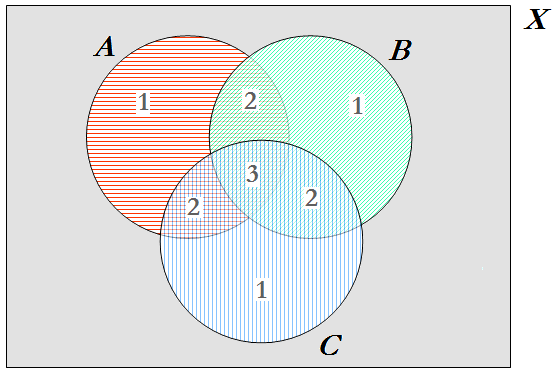
\includegraphics[width=\textwidth]{venn}
    \caption{Venn diagram}
    \label{fig:Figure2}
  \end{subfigure}
  \caption{Best Pictures}
  \label{fig:animations}
\end{figure}

\end{landscape}

\section{Third section}

\tochide\section{Hidden section}




%*******************************************************************************
%*********************************** Third Chapter *****************************
%*******************************************************************************


\chapter{My third chapter}  %Title of the Third Chapter

\ifpdf
    \graphicspath{{Chapter3/Figs/Raster/}{Chapter3/Figs/PDF/}{Chapter3/Figs/}}
\else
    \graphicspath{{Chapter3/Figs/Vector/}{Chapter3/Figs/}}
\fi


%********************************** %First Section  **************************************
\section{Title with math \texorpdfstring{$\sigma$}{[sigma]}} %Section - 1.1

The well known Pythagorean theorem \(x^2 + y^2 = z^2\) was
proved to be invalid for other exponents.
Meaning the next equation has no integer solutions:
$x^n + y^n = z^n.$

The binomial coefficient is defined by the next expression:
\[
    \binom{n}{k} = \frac{n!}{k!(n-k)!}
\]

And of course this command can be included in the normal
text flow \(\binom{n}{k}\). Limit $\lim_{x\to\infty} f(x)$ inside text.
$$\lim_{x\to\infty} f(x)$$

The most famous equation in the world: $E^2 = (m_0c^2)^2 + (pc)^2$, which is
known as the \textbf{energy-mass-momentum} relation as an in-line equation.

\begin{align}
CIF: \hspace*{5mm}F_0^j(a) = \frac{1}{2\pi \iota} \oint_{\gamma} \frac{F_0^j(z)}{z - a} dz
\end{align}

Integral $\int_{a}^{b} x^2 dx$ inside text.

\begin{align}
\iiint_V \mu(u,v,w) \,du\,dv\,dw
\end{align}


%********************************** %Second Section  *************************************
\section{Preliminaries I. Free constructions} %Section - 1.2

We will work with point-free real numbers as they are usually described in literature, that is, by generators subject to relations. Since the free generators come from a set that is in fact a meet-semilattice (while its elements are used in the free construction simply as elements of a set) we think that it may be useful for the reader to compare the free frames over sets with free frames over semilattices.

We will work with point-free real numbers as they are usually described in literature, that is, by generators subject to relations. Since the free generators come from a set that is in fact a meet-semilattice (while its elements are used in the free construction simply as elements of a set) we think that it may be useful for the reader to compare the free frames over sets with free frames over semilattices.



\subsection{Free semilattice with 1.} For a set $X$ define
$
F(X)=\{A\subseteq X\mid A\ \text{finite}\}
$
ordered by $\leq\;=\;\supseteq$ so that we have the meet $A\wedge B=A\cup B$. Denote by $\beta_X$ the mapping
$$
\beta_X=(x\mapsto\{x\})\colon X\to F(X).
$$
 Then we have for each meet-semilattice $S$ with 1 and each mapping $f\colon X\to S$ precisely one meet-semilattice homomorphism $\overline{f}\colon F(X)\to S$ such that $\overline{f}\beta_X=f$ and $\overline{f}(\emptyset)=1$, namely the homomorphism defined by $\overline{f}(A)=\bigwedge_{x\in A} f(x)$.

\subsection{Free frame generated by a semilattice with 1.} For a meet-semilattice  $S$ with 1  set
$
{\mathfrak D}(S)=\{U\subseteq S\mid\downarrow\! U=U\neq \emptyset\}.
$
${\mathfrak D}(S)$ is a frame with unions for joins and intersections for meets and if we denote by $\alpha_S$ the mapping
$$
\alpha_S=(s\mapsto\downarrow\! s)\colon S\to {\mathfrak D}(S)
$$
we have a meet-semilattice homomorphism such that for each frame $L$ and each meet-semilattice homomorphism $h\colon S\to L$ there is precisely one frame  homomorphism $\widehat h\colon {\mathfrak D}(S)\to L$ such that $\widehat h\alpha_S=h$, namely that defined by $\widehat h(U)=\bigvee_{s\in U}h(s)$.

The free frame over a set can be now obtained combining $F$ and $\mathfrak D$, that is, as $\mathfrak{D}F(X)$.

\subsection{Free frames over a set and over a meet-semilattice compared.}
Well, one may go on adding more and more subsections, but these are enough to illustrate how this works!


%********************************** % Third Section  *************************************
\section{Where does it come from?}  %Section - 1.3
\label{section1.3}

And this illustrates how one may add more sections to the text.


 \section{Next section}

 \section{Next section}



\chapter{Conclusion}

% **************************** Define Graphics Path **************************
\ifpdf
    \graphicspath{{Chapter4/Figs/Raster/}{Chapter4/Figs/PDF/}{Chapter4/Figs/}}
\else
    \graphicspath{{Chapter4/Figs/Vector/}{Chapter4/Figs/}}
\fi

%\section{First section of the fourth chapter}
We end with some final comments \dots



%\include{Chapter5/chapter5}
%\include{Chapter6/chapter6}
%\include{Chapter7/chapter7}



% ********************************** Back Matter *******************************
%% Backmatter should be commented out, if you are using appendices after References

%\backmatter

% ********************************** Bibliography ******************************
\begin{spacing}{0.9}

% To use the conventional natbib style referencing
% Bibliography style previews: http://nodonn.tipido.net/bibstyle.php
% Reference styles: http://sites.stat.psu.edu/~surajit/present/bib.htm

\bibliographystyle{apalike}
%\bibliographystyle{plainnat} % use this to have URLs listed in References
\cleardoublepage
\bibliography{References/references} % Path to your References.bib file


% If you would like to use BibLaTeX for your references, pass `custombib' as
% an option in the document class. The location of 'reference.bib' should be
% specified in the preamble.tex file in the custombib section.
% Comment out the lines related to natbib above and uncomment the following line.

%\printbibliography[heading=bibintoc, title={References}]


\end{spacing}

% ********************************** Appendices ********************************

\begin{appendices} % Using appendices environment

% ******************************* Thesis Appendix A ********************************
\chapter{More information $\int$}

\section*{Carl Friedrich Gauss}

Johann Carl Friedrich Gauss (30 April 1777 -- 23 February 1855) was a German mathematician who contributed significantly to many fields, including number theory, algebra, statistics, analysis, differential geometry, geodesy, geophysics, electrostatics, astronomy, matrix theory, and optics.

Sometimes referred to as the Princeps mathematicorum (Latin, ``the Prince of Mathematicians'' or ``the foremost of mathematicians'') and ``greatest mathematician since antiquity'', Gauss had a remarkable influence in many fields of mathematics and science and is ranked as one of history's most influential mathematicians.

Gauss was a child prodigy. There are many anecdotes about his precocity while a toddler, and he made his first ground-breaking mathematical discoveries while still a teenager. He completed Disquisitiones Arithmeticae, his magnum opus, in 1798 at the age of 21, though it was not published until 1801. This work was fundamental in consolidating number theory as a discipline and has shaped the field to the present day.

Gauss's intellectual abilities attracted the attention of the Duke of Brunswick, who sent him to the Collegium Carolinum (now Braunschweig University of Technology), which he attended from 1792 to 1795, and to the University of G\"{o}ttingen from 1795 to 1798. While at university, Gauss independently rediscovered several important theorems; his breakthrough occurred in 1796 when he showed that any regular polygon with a number of sides which is a Fermat prime (and, consequently, those polygons with any number of sides which is the product of distinct Fermat primes and a power of 2) can be constructed by compass and straightedge. This was a major discovery in an important field of mathematics; construction problems had occupied mathematicians since the days of the Ancient Greeks, and the discovery ultimately led Gauss to choose mathematics instead of philology as a career. Gauss was so pleased by this result that he requested that a regular heptadecagon be inscribed on his tombstone. The stonemason declined, stating that the difficult construction would essentially look like a circle.

The year 1796 was most productive for both Gauss and number theory. He discovered a construction of the heptadecagon on 30 March. He further advanced modular arithmetic, greatly simplifying manipulations in number theory. On 8 April he became the first to prove the quadratic reciprocity law. This remarkably general law allows mathematicians to determine the solvability of any quadratic equation in modular arithmetic. The prime number theorem, conjectured on 31 May, gives a good understanding of how the prime numbers are distributed among the integers.

\section*{Another section}

\subsection*{Subsection}

\subsubsection*{Subsubsection}
...


\end{appendices}


% *************************************** General Index ********************************
\printthesisindex % If index is present


\end{document}
